% Self-contained, editable vector recreation. Compile with pdflatex.
\documentclass{article}
\usepackage[paperwidth=17.8cm,paperheight=26.8cm,margin=.22cm]{geometry}
\usepackage{amsmath,tikz,xcolor}
\usetikzlibrary{arrows.meta,shapes.geometric}
\pagestyle{empty}\setlength{\parindent}{0pt}
\definecolor{navy}{HTML}{10224F}\definecolor{blue}{HTML}{1769D2}
\definecolor{cyan}{HTML}{DFF5FB}\definecolor{cyanline}{HTML}{25B8DB}
\definecolor{orange}{HTML}{E87513}\definecolor{peach}{HTML}{FFF1DE}
\definecolor{teal}{HTML}{078C91}\definecolor{red}{HTML}{D83F35}
\tikzset{
  bp/.style={draw=cyanline,fill=cyan,very thick,rounded corners=2mm},
  op/.style={draw=orange,fill=peach,very thick,rounded corners=2mm},
  wb/.style={draw=blue!60,fill=white,rounded corners=1mm,line width=.5pt},
  ob/.style={draw=orange!75,fill=white,rounded corners=1mm,line width=.5pt},
  tb/.style={draw=teal!75,fill=white,rounded corners=1mm,line width=.5pt},
  arr/.style={-Latex,draw=blue,line width=1.2pt},
  int/.style={-Latex,draw=orange,line width=1.2pt},
  tiny/.style={font=\sffamily\fontsize{5.1}{6.2}\selectfont,text=navy},
  body/.style={font=\sffamily\fontsize{6.2}{7.4}\selectfont,text=navy},
  lab/.style={font=\sffamily\fontsize{7}{8.2}\bfseries\selectfont,text=navy}}
\newcommand{\ttl}[2]{\node[anchor=north west,font=\sffamily\fontsize{9}{10.3}\bfseries\selectfont,text=navy] at (.65,.45) {#1\quad #2};}
\newcommand{\grid}[3]{\foreach \gx in {0,...,4}{\foreach \gy in {0,...,3}{\draw[draw=blue!50,fill=#3] (#1+\gx*.43,#2+\gy*.43) rectangle ++(.4,.4);}}}
\newcommand{\bars}[3]{\draw[blue!50] (#1,#2)--(#1+4.4,#2);\foreach \xx/\hh in {0/2.65,1/1.5,2/.95,3/.6}{\fill[blue!70] (#1+\xx+.15,#2) rectangle (#1+\xx+.72,#2-\hh);}\node[tiny,anchor=north] at (#1+2.2,#2+.15) {#3};}
\begin{document}\noindent
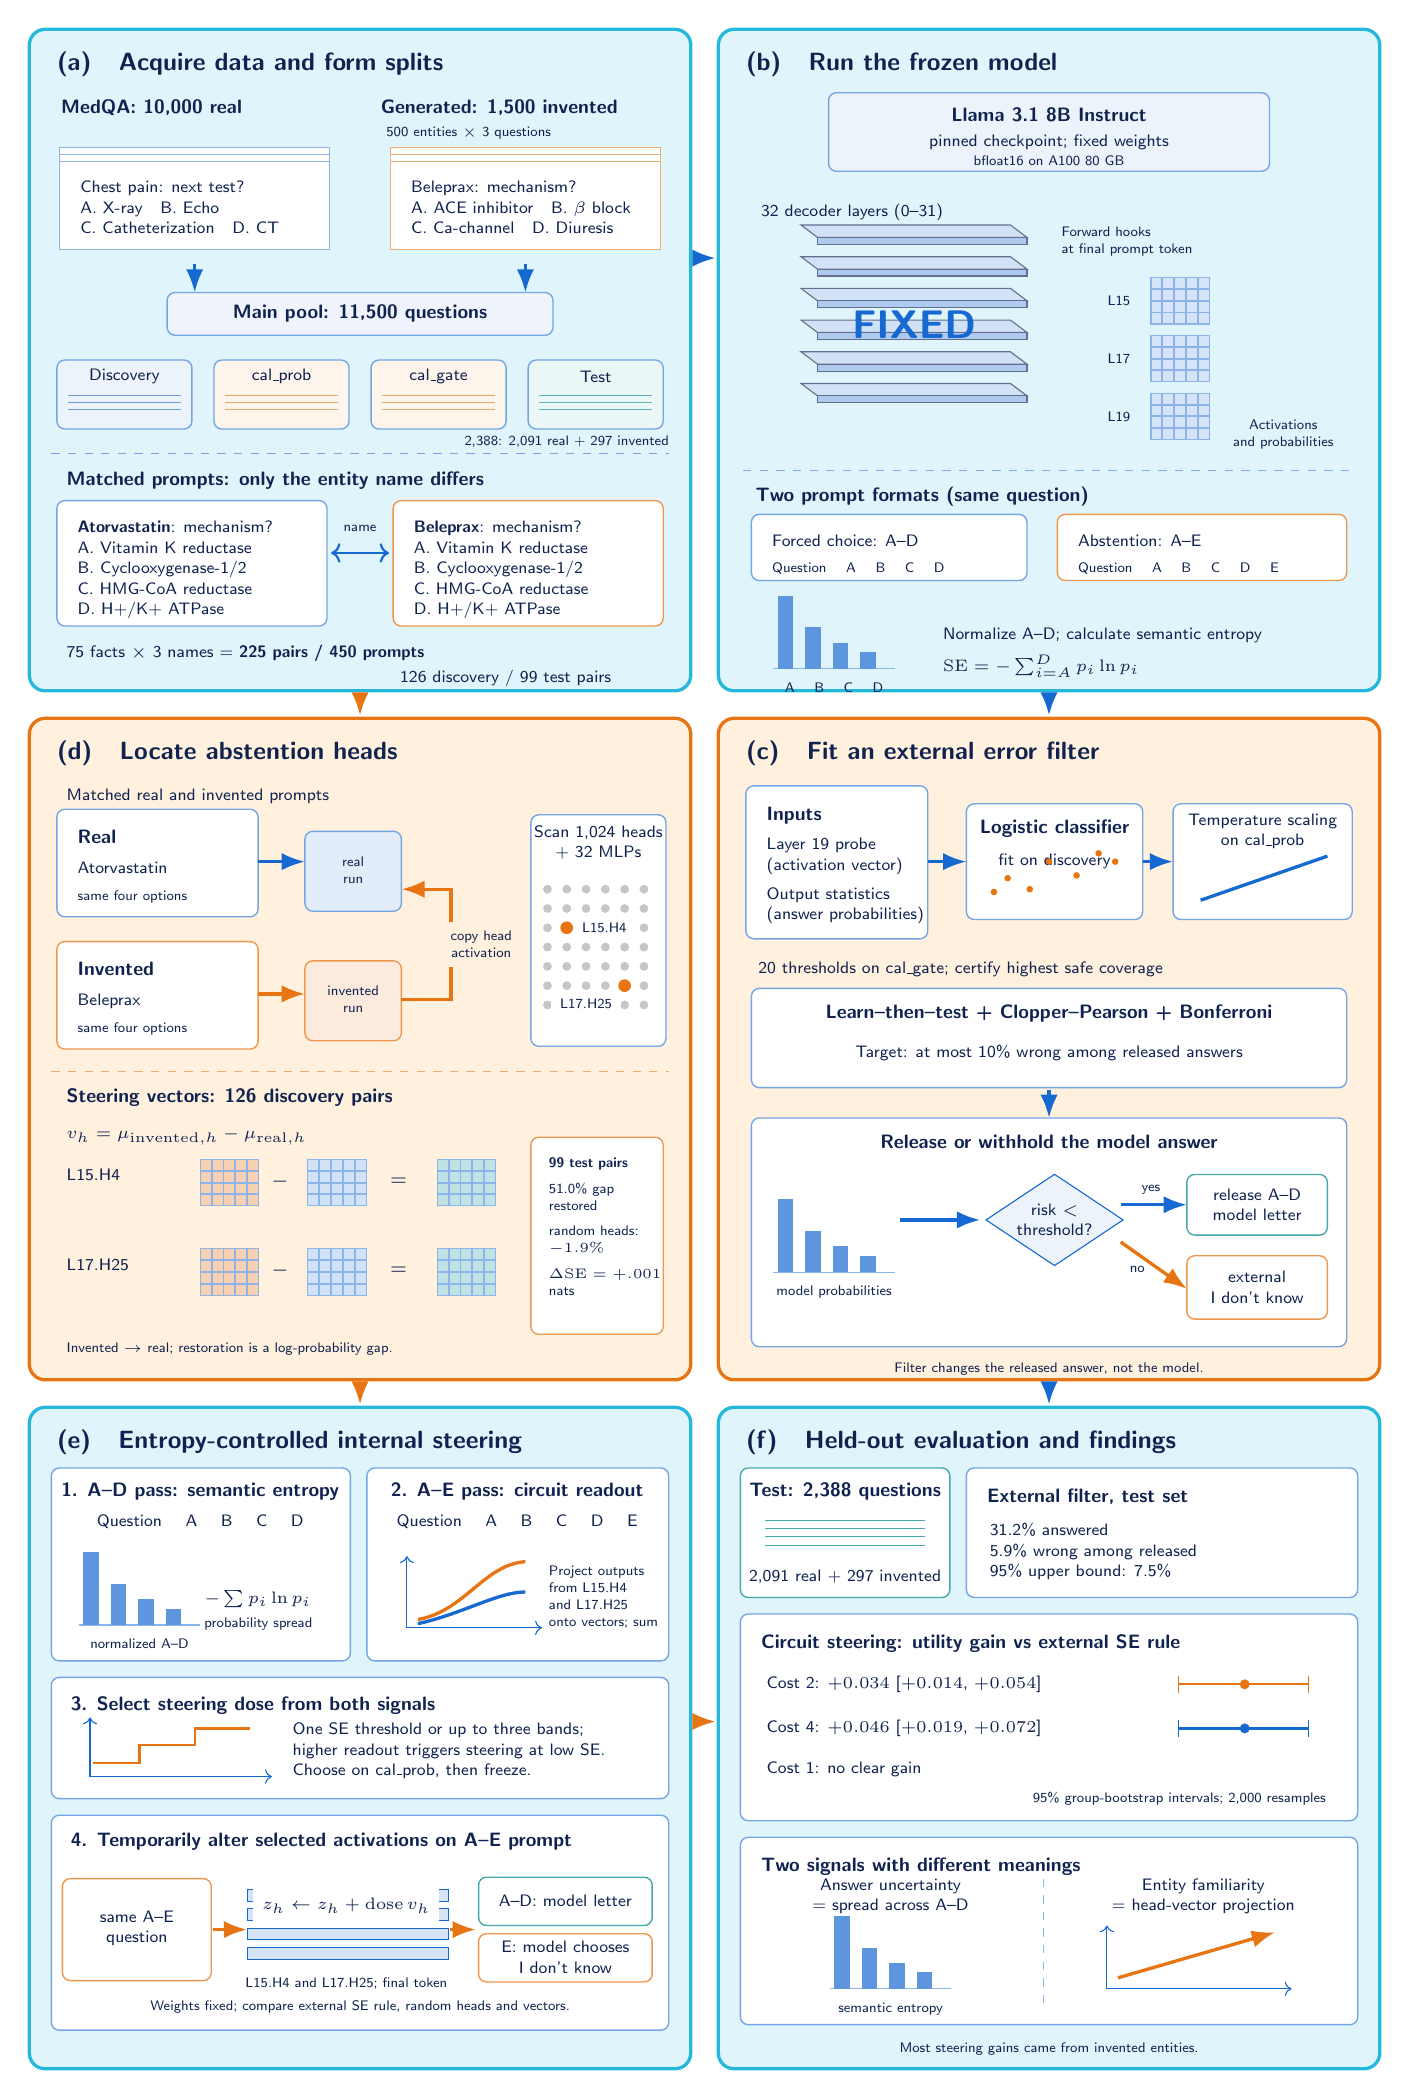
\begin{tikzpicture}[x=.35cm,y=-.35cm,every node/.style={font=\sffamily\fontsize{6.2}{7.4}\selectfont,text=navy}]
% (a) Main pool, splits, and the separate matched-pair set.
\begin{scope}
\draw[bp] (0,0) rectangle (24,24);\ttl{(a)}{Acquire data and form splits}
\node[lab,anchor=north west] at (.8,2.2) {MedQA: 10,000 real};
\node[lab,anchor=north west] at (12.4,2.2) {Generated: 1,500 invented};
\node[tiny,anchor=north west] at (12.6,3.2) {500 entities $\times$ 3 questions};
\foreach \y in {4.3,4.55,4.8}{\draw[fill=white,draw=blue!50] (1.1,\y) rectangle (10.9,\y+3.2);\draw[fill=white,draw=orange!60] (13.1,\y) rectangle (22.9,\y+3.2);}
\node[body,align=left,anchor=north west] at (1.5,5.15) {Chest pain: next test?\\A. X-ray\quad B. Echo\\C. Catheterization\quad D. CT};
\node[body,align=left,anchor=north west] at (13.5,5.15) {Beleprax: mechanism?\\A. ACE inhibitor\quad B. $\beta$ block\\C. Ca-channel\quad D. Diuresis};
\draw[arr] (6,8.5)--(6,9.55);\draw[arr] (18,8.5)--(18,9.55);
\draw[wb,fill=blue!7] (5,9.55) rectangle (19,11.1);
\node[lab] at (12,10.3) {Main pool: 11,500 questions};
\foreach \x/\name/\col in {1/Discovery/blue,6.7/cal\_prob/orange,12.4/cal\_gate/orange,18.1/Test/teal}{
\draw[wb,fill=\col!8] (\x,12) rectangle (\x+4.9,14.5);
\foreach \y in {13.3,13.55,13.8}{\draw[\col!65] (\x+.4,\y)--(\x+4.5,\y);}
\node[body] at (\x+2.45,12.6) {\name};}
\node[tiny,anchor=north] at (19.5,14.4) {2,388: 2,091 real + 297 invented};
\draw[dashed,blue!60] (.8,15.4)--(23.2,15.4);
\node[lab,anchor=north west] at (1,15.7) {Matched prompts: only the entity name differs};
\draw[wb] (1,17.1) rectangle (10.8,21.65);\draw[ob] (13.2,17.1) rectangle (23,21.65);
\node[body,align=left,anchor=north west] at (1.4,17.5) {\textbf{Atorvastatin}: mechanism?\\A. Vitamin K reductase\\B. Cyclooxygenase-1/2\\C. HMG-CoA reductase\\D. H+/K+ ATPase};
\node[body,align=left,anchor=north west] at (13.6,17.5) {\textbf{Beleprax}: mechanism?\\A. Vitamin K reductase\\B. Cyclooxygenase-1/2\\C. HMG-CoA reductase\\D. H+/K+ ATPase};
\draw[<->,blue,thick] (10.95,19)--(13.05,19);
\node[tiny,fill=cyan] at (12,18.1) {name};
\node[body,anchor=north west] at (1,22) {75 facts $\times$ 3 names = \textbf{225 pairs / 450 prompts}};
\node[body,anchor=north west] at (13.1,22.9) {126 discovery / 99 test pairs};
\end{scope}
% (b) Pinned frozen checkpoint and two different prompt formats.
\begin{scope}[shift={(25,0)}]
\draw[bp] (0,0) rectangle (24,24);\ttl{(b)}{Run the frozen model}
\draw[wb,fill=blue!8] (4,2.3) rectangle (20,5.15);
\node[lab] at (12,3.1) {Llama 3.1 8B Instruct};
\node[body] at (12,4.1) {pinned checkpoint; fixed weights};
\node[tiny] at (12,4.78) {bfloat16 on A100 80 GB};
\node[body,anchor=north west] at (1.2,6) {32 decoder layers (0--31)};
\foreach \y in {7.1,8.25,9.4,10.55,11.7,12.85}{\draw[fill=blue!20,draw=navy!65] (3,\y)--(10.6,\y)--(11.2,\y+.45)--(3.6,\y+.45)--cycle;\draw[fill=blue!35,draw=navy!65] (3.6,\y+.45) rectangle (11.2,\y+.7);}
\node[font=\sffamily\fontsize{15}{15}\bfseries\selectfont,text=blue] at (7.1,10.7) {FIXED};
\node[tiny,align=left,anchor=north west] at (12.1,6.8) {Forward hooks\\at final prompt token};
\foreach \y/\name in {9/L15,11.1/L17,13.2/L19}{\grid{15.7}{\y}{blue!18}\node[tiny,anchor=east] at (15.3,\y+.85) {\name};}
\node[tiny,align=center] at (20.5,14.7) {Activations\\and probabilities};
\draw[dashed,blue!55] (.9,16)--(23.1,16);
\node[lab,anchor=north west] at (1,16.25) {Two prompt formats (same question)};
\draw[wb] (1.2,17.6) rectangle (11.2,20);
\node[body,anchor=north west] at (1.6,18) {Forced choice: A--D};
\node[tiny,anchor=north west] at (1.6,19) {Question \quad A \quad B \quad C \quad D};
\draw[ob] (12.3,17.6) rectangle (22.8,20);
\node[body,anchor=north west] at (12.7,18) {Abstention: A--E};
\node[tiny,anchor=north west] at (12.7,19) {Question \quad A \quad B \quad C \quad D \quad E};
\bars{2}{23.2}{A \quad B \quad C \quad D}
\node[body,anchor=north west] at (7.8,21.35) {Normalize A--D; calculate semantic entropy};
\node[body,anchor=north west] at (7.8,22.35) {$\mathrm{SE}=-\sum_{i=A}^{D}p_i\ln p_i$};
\end{scope}
% (d) Activation patching identifies heads and steering directions.
\begin{scope}[shift={(0,25)}]
\draw[op] (0,0) rectangle (24,24);\ttl{(d)}{Locate abstention heads}
\node[body,anchor=north west] at (1,2.2) {Matched real and invented prompts};
\draw[wb] (1,3.3) rectangle (8.3,7.2);
\node[lab,anchor=north west] at (1.4,3.7) {Real};
\node[body,anchor=north west] at (1.4,4.85) {Atorvastatin};
\node[tiny,anchor=north west] at (1.4,5.9) {same four options};
\draw[ob] (1,8.1) rectangle (8.3,12);
\node[lab,anchor=north west] at (1.4,8.5) {Invented};
\node[body,anchor=north west] at (1.4,9.65) {Beleprax};
\node[tiny,anchor=north west] at (1.4,10.7) {same four options};
\draw[wb,fill=blue!12] (10,4.1) rectangle (13.5,7);
\draw[ob,fill=orange!15] (10,8.8) rectangle (13.5,11.7);
\node[tiny,align=center] at (11.75,5.5) {real\\run};
\node[tiny,align=center] at (11.75,10.2) {invented\\run};
\draw[arr] (8.3,5.2)--(10,5.2);\draw[int] (8.3,10)--(10,10);
\draw[int] (13.5,10.2)--(15.3,10.2)--(15.3,6.2)--(13.5,6.2);
\node[tiny,fill=peach,align=center] at (16.4,8.2) {copy head\\activation};
\draw[wb] (18.2,3.5) rectangle (23.1,11.9);
\node[body,align=center] at (20.65,4.5) {Scan 1,024 heads\\+ 32 MLPs};
\foreach \xx in {18.8,19.5,...,22.3}{\foreach \yy in {6.2,6.9,...,10.4}{\fill[gray!45] (\xx,\yy) circle (.16);}}
\fill[orange] (19.5,7.6) circle (.23);\fill[orange] (21.6,9.7) circle (.23);
\node[tiny,fill=white,anchor=west] at (19.7,7.6) {L15.H4};
\node[tiny,fill=white,anchor=east] at (21.5,10.35) {L17.H25};
\draw[dashed,orange!60] (.8,12.8)--(23.2,12.8);
\node[lab,anchor=north west] at (1,13.1) {Steering vectors: 126 discovery pairs};
\node[body,anchor=north west] at (1,14.5) {$v_h=\mu_{\mathrm{invented},h}-\mu_{\mathrm{real},h}$};
\foreach \yy/\name in {16/L15.H4,19.25/L17.H25}{
\node[body,anchor=north west] at (1,\yy) {\name};
\grid{6.2}{\yy}{orange!33}\node[lab] at (9.1,\yy+.8) {$-$};
\grid{10.1}{\yy}{blue!20}\node[lab] at (13.4,\yy+.8) {$=$};
\grid{14.8}{\yy}{teal!25}}
\draw[ob] (18.2,15.2) rectangle (23,22.35);
\node[tiny,align=left,anchor=north west] at (18.5,15.6) {\textbf{99 test pairs}\\[3pt]51.0\% gap\\restored\\[3pt]random heads:\\$-1.9\%$\\[3pt]$\Delta\mathrm{SE}=+.001$\\nats};
\node[tiny,anchor=north west] at (1,22.3) {Invented $\rightarrow$ real; restoration is a log-probability gap.};
\end{scope}
% (c) External error filter; no intervention in the language model.
\begin{scope}[shift={(25,25)}]
\draw[op] (0,0) rectangle (24,24);\ttl{(c)}{Fit an external error filter}
\draw[wb] (1,2.45) rectangle (7.6,8);
\node[lab,anchor=north west] at (1.4,2.85) {Inputs};
\node[body,align=left,anchor=north west] at (1.4,4) {Layer 19 probe\\(activation vector)\\[3pt]Output statistics\\(answer probabilities)};
\draw[arr] (7.6,5.2)--(9,5.2);
\draw[wb] (9,3.1) rectangle (15.4,7.3);
\node[lab,align=center] at (12.2,4) {Logistic classifier};
\node[body] at (12.2,5.2) {fit on discovery};
\foreach \xx/\yy in {10/6.3,10.5/5.8,11.3/6.2,12/5.2,13/5.7,13.8/4.9,14.4/5.2}{\fill[orange] (\xx,\yy) circle (.12);}
\draw[arr] (15.4,5.2)--(16.5,5.2);
\draw[wb] (16.5,3.1) rectangle (23,7.3);
\node[body,align=center] at (19.75,4.1) {Temperature scaling\\on cal\_prob};
\draw[blue,very thick] (17.5,6.6)--(22.1,5);
\node[body,anchor=north west] at (1.1,8.5) {20 thresholds on cal\_gate; certify highest safe coverage};
\draw[wb] (1.2,9.8) rectangle (22.8,13.4);
\node[lab] at (12,10.7) {Learn--then--test + Clopper--Pearson + Bonferroni};
\node[body] at (12,12.15) {Target: at most 10\% wrong among released answers};
\draw[arr] (12,13.5)--(12,14.5);
\draw[wb] (1.2,14.5) rectangle (22.8,22.8);
\node[lab] at (12,15.35) {Release or withhold the model answer};
\bars{2}{20.1}{model probabilities}
\draw[arr] (6.6,18.2)--(9.5,18.2);
\node[diamond,draw=blue,fill=blue!8,aspect=1.5,inner sep=1pt,body,align=center] at (12.2,18.2) {risk $<$\\threshold?};
\draw[arr] (14.6,17.65)--(17,17.65);
\node[tiny] at (15.7,17.1) {yes};
\draw[tb] (17,16.55) rectangle (22.1,18.75);
\node[body,align=center] at (19.55,17.65) {release A--D\\model letter};
\draw[int] (14.6,19)--(17,20.7);
\node[tiny] at (15.2,20) {no};
\draw[ob] (17,19.5) rectangle (22.1,21.8);
\node[body,align=center] at (19.55,20.65) {external\\I don't know};
\node[tiny,anchor=north] at (12,23.05) {Filter changes the released answer, not the model.};
\end{scope}
% (e) Entropy and head readout are separate unsteered passes.
\begin{scope}[shift={(0,50)}]
\draw[bp] (0,0) rectangle (24,24);\ttl{(e)}{Entropy-controlled internal steering}
\draw[wb] (.8,2.2) rectangle (11.65,9.2);
\node[lab] at (6.2,3.05) {1. A--D pass: semantic entropy};
\node[body] at (6.2,4.15) {Question \quad A \quad B \quad C \quad D};
\bars{1.8}{7.9}{normalized A--D}
\node[body,anchor=north west] at (6,6.3) {$-\sum p_i\ln p_i$};
\node[tiny,anchor=north west] at (6,7.3) {probability spread};
\draw[wb] (12.25,2.2) rectangle (23.2,9.2);
\node[lab] at (17.7,3.05) {2. A--E pass: circuit readout};
\node[body] at (17.7,4.15) {Question \quad A \quad B \quad C \quad D \quad E};
\draw[->,blue] (13.7,8)--(13.7,5.4);\draw[->,blue] (13.7,8)--(18.6,8);
\draw[orange,very thick] (14.1,7.7).. controls (15.8,7.4) and (16.5,5.7).. (18,5.6);
\draw[blue,very thick] (14.1,7.85).. controls (15.7,7.5) and (17,6.7).. (18,6.7);
\node[tiny,align=left,anchor=north west] at (18.5,5.4) {Project outputs\\from L15.H4\\and L17.H25\\onto vectors; sum};
\draw[wb] (.8,9.8) rectangle (23.2,14.2);
\node[lab,anchor=north west] at (1.15,10.15) {3. Select steering dose from both signals};
\draw[->,blue] (2.2,13.4)--(8.8,13.4);\draw[->,blue] (2.2,13.4)--(2.2,11.25);
\draw[orange,thick] (2.3,12.9)--(4,12.9)--(4,12.25)--(6,12.25)--(6,11.65)--(8,11.65);
\node[body,align=left,anchor=north west] at (9.2,11.1) {One SE threshold or up to three bands;\\higher readout triggers steering at low SE.\\Choose on cal\_prob, then freeze.};
\draw[wb] (.8,14.8) rectangle (23.2,22.6);
\node[lab,anchor=north west] at (1.15,15.1) {4. Temporarily alter selected activations on A--E prompt};
\draw[ob] (1.2,17.1) rectangle (6.6,20.8);
\node[body,align=center] at (3.9,18.9) {same A--E\\question};
\draw[int] (6.65,18.95)--(7.9,18.95);
\foreach \yy in {17.5,18.2,18.9,19.6}{\draw[fill=blue!18,draw=blue] (7.9,\yy) rectangle (15.2,\yy+.42);}
\node[body,fill=white] at (11.5,18.1) {$z_h\leftarrow z_h+\mathrm{dose}\,v_h$};
\node[tiny,anchor=north] at (11.5,20.35) {L15.H4 and L17.H25; final token};
\draw[int] (15.25,18.95)--(16.2,18.95);
\draw[tb] (16.3,17.05) rectangle (22.6,18.8);
\node[body] at (19.45,17.9) {A--D: model letter};
\draw[ob] (16.3,19.1) rectangle (22.6,20.85);
\node[body,align=center] at (19.45,19.95) {E: model chooses\\I don't know};
\node[tiny,anchor=north] at (12,21.2) {Weights fixed; compare external SE rule, random heads and vectors.};
\end{scope}
% (f) Both branches meet only at held-out evaluation.
\begin{scope}[shift={(25,50)}]
\draw[bp] (0,0) rectangle (24,24);\ttl{(f)}{Held-out evaluation and findings}
\draw[tb] (.8,2.2) rectangle (8.4,6.9);
\node[lab] at (4.6,3.05) {Test: 2,388 questions};
\foreach \yy in {4.1,4.4,4.7,5}{\draw[teal!75] (1.7,\yy)--(7.5,\yy);}
\node[body] at (4.6,6.15) {2,091 real + 297 invented};
\draw[wb] (9,2.2) rectangle (23.2,6.9);
\node[lab,anchor=north west] at (9.4,2.6) {External filter, test set};
\node[body,align=left,anchor=north west] at (9.5,3.85) {31.2\% answered\\5.9\% wrong among released\\95\% upper bound: 7.5\%};
\draw[wb] (.8,7.5) rectangle (23.2,15);
\node[lab,anchor=north west] at (1.2,7.9) {Circuit steering: utility gain vs external SE rule};
\foreach \yy/\labname/\est/\lo/\hi/\col in {10.05/Cost 2/0.034/0.014/0.054/orange,11.65/Cost 4/0.046/0.019/0.072/blue}{
\node[body,anchor=west] at (1.4,\yy) {\labname: $+\est$ [$+\lo$, $+\hi$]};
\draw[\col,thick] (16.7,\yy)--(21.4,\yy);
\draw[\col] (16.7,\yy-.3)--(16.7,\yy+.3);
\draw[\col] (21.4,\yy-.3)--(21.4,\yy+.3);
\fill[\col] (19.1,\yy) circle (.18);}
\node[body,anchor=west] at (1.4,13.15) {Cost 1: no clear gain};
\node[tiny,anchor=east] at (22.4,14.2) {95\% group-bootstrap intervals; 2,000 resamples};
\draw[wb] (.8,15.6) rectangle (23.2,22.4);
\node[lab,anchor=north west] at (1.2,16) {Two signals with different meanings};
\draw[dashed,blue!50] (11.8,17.1)--(11.8,21.9);
\node[body,align=center] at (6.25,17.75) {Answer uncertainty\\= spread across A--D};
\bars{4.05}{21.1}{semantic entropy}
\node[body,align=center] at (17.6,17.75) {Entity familiarity\\= head-vector projection};
\draw[->,blue] (14.1,21.1)--(20.8,21.1);
\draw[->,blue] (14.1,21.1)--(14.1,18.8);
\draw[orange,very thick,-Latex] (14.5,20.7)--(20.2,19.05);
\node[tiny,anchor=north] at (12,22.7) {Most steering gains came from invented entities.};
\end{scope}
% Reading order and distinct branches.
\draw[arr] (24.1,8.3)--(24.9,8.3);
\draw[int] (12,24.1)--(12,24.9);
\draw[arr] (37,24.1)--(37,24.9);
\draw[int] (12,49.1)--(12,49.9);
\draw[arr] (37,49.1)--(37,49.9);
\draw[int] (24.1,61.4)--(24.9,61.4);
\end{tikzpicture}
\end{document}
